\subsection{Results}\label{sec:results}

% <<<<<<< HEAD
% This section presents the results of our research. In Section~\ref{sec:ml}, we compare the performance of various machine learning (ML) algorithms in classifying apps from the \fds dataset as either malware or non-malware using our framework, \droidxpflow. In Section~\ref{sec:family-assessment}, we evaluate the performance of our approach, focusing on malware families and assessing the accuracy of detecting each of them. Finally, in Section~\ref{sec:new-mas-approach}, we provide an overview of the results obtained with our approach and compare them to existing state-of-the-art method.
% =======



In this section we present the results of our research.
First we compare the performance of different ML algorithms in classifying
as malware or non-malware the repackaged version of the apps in the \fds (Section~\ref{sec:ml}) using \droidxpflow.
Recall that previous research employed the \emph{vanilla}
\mas, which relies solely on calls to sensitive APIs for app classification. Our previous
research showed that the performance of the vanilla \mas is compromised when considering
the \cds, in particular due to samples from specific malware families (i.e., \gps, \rmb, \dwg, and \tjk families).
In Section~\ref{sec:comparation}, we present the gains in classification performance when combining
the \mas with \droidxpflow; while, in Section~\ref{sec:family-assessment}, we show to which extent
\droidxpflow correctly clasifies the malware families for which the \mas approach
present the worst accuracy in our previous study.

\subsubsection{Comparison of Machine Learning Algorithms}\label{sec:ml}

As discussed in Section~\ref{sec:droidxpflow}, \droidxpflow extends \droidxp to collect network
flow information from apps during test case generation campaigns. To answer our fitst research question,
we conduct an experiment that compares the performance of various ML algorithms using our \fds dataset with all the features (1,640)
for malware classification. This stage of our research considers the following ML algorithms:

\rb{Seria legal justificarmos o poru\^{e} da escolha desses algoritmos, e nao de outros (como SVM). Talvez o Prof. Eduardo possa ajudar aqui.}

\begin{itemize}
 \item Logistic Regression (LR)
 \item Linear Discriminant Analysis (LDA)
 \item Quadratic Discriminant Analysis (QDA)
 \item Random Forest (RF)
\end{itemize}

\rb{As configuracoes dos parametros que foram explorados deveriam estar descritas nas secoes anteriores; antes de results.}

In this research we also explore the Energy-Based Flow Classifier (EFC), which has been used for intrusion and botnet detection using
network flows~\cite{DBLP:journals/tnsm/PontesSGBM21}. For our experiments using the \fds, we separate $70\%$ of the samples ($2,847$) for
training, and $30\%$ ($1,220$ samples) for testing. To equalize the performance of each ML algorithm, we evaluated them using the default parameter values for each method.
Ultimately, the RF algorithm outperformed the others when evaluated with standard metrics (recall, precision, F1-score, and Area Under the Curve (AUC)). RF algorithm aggregates multiple decision trees,
with each tree constructed using a random subset of features. This process decorrelates the trees, allowing for a more thorough
exploration of the model and substantially improving predictive performance~\cite{james2023introduction}.
Table~\ref{tab:ml-metrics} presents the results. 

\begin{table}[htb]
    \caption{Accuracy of the ML algorithms to classify the app as malware or non-malware using network flow data from the \fds.}
\centering{
    \begin{tabular}{lrrrr} \toprule
    Algorithm & Precision & Recall & \fone & AUC \\ \midrule 
    LR  & 0.74 & 0.98 & 0.84 & 0.74 \\
    LDA & 0.77 & 0.86 & 0.82 & 0.82 \\
    QDA & 0.73 & 0.54 & 0.62 & 0.79 \\
    EFC & 0.75 & 0.97 & 0.85 & 0.66 \\
    RF & 0.76 & 0.97 & 0.86 & 0.94 \\ \bottomrule    
    \end{tabular}
} \label{tab:ml-metrics}
\end{table}

\begin{finding}
  The RF algorithm outperforms the others popular classification algorithms, achieving higher values across the metrics explored (recall, precision, \fone, and Area Under the Curve).
\end{finding}

In what follows, when we present the accuracy of \droidxpflow, we
will be describing its usage with the Random Forest algotithm.


% \begin{figure*}[h]
%   \centering  
%     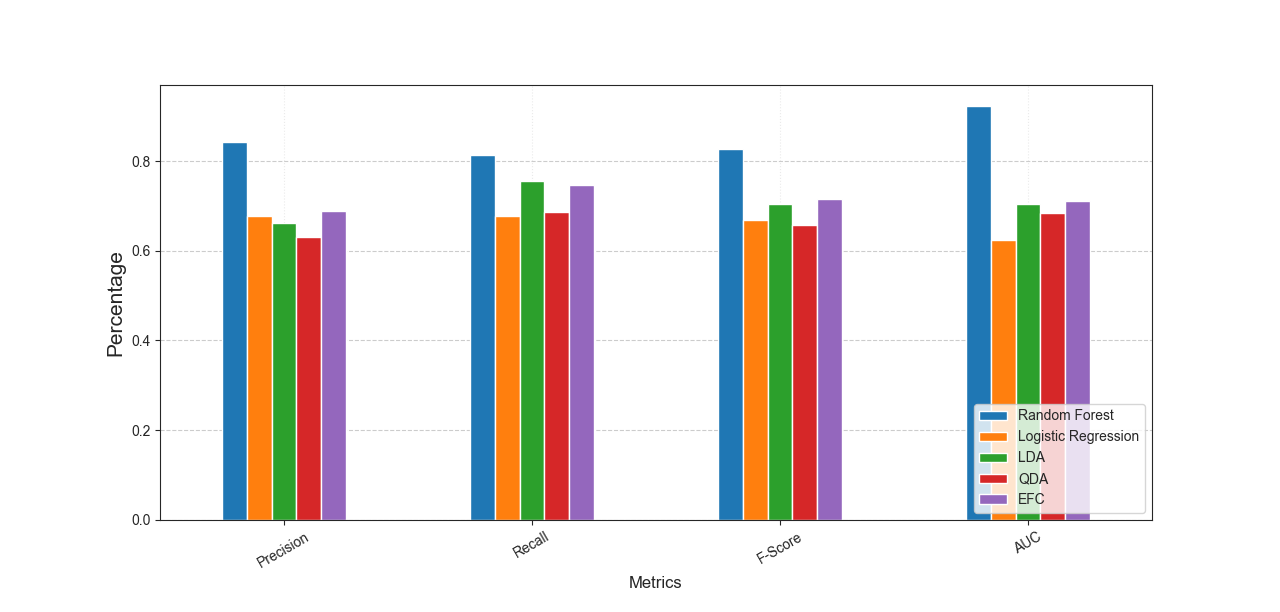
\includegraphics[width=0.85\textwidth]{image/barGraphMetrics.png} \\[\abovecaptionskip]
%   \caption{The comparison of machine learning algorithms}\label{fig:metrics}
% \end{figure*}

\subsubsection{A comparison between \droidxpflow and the \mas}\label{sec:comparation}

Here we compare the accuracy performance of \droidxpflow and the \mas classifiers.
Our comparison here also relies on standard metrics
(recall, precision, and F1-score), and we present the results using the
same $30\%$ of samples (1,220) from the \fds dataset that we used for the tests
in Section~\ref{sec:ml}. However, this time we used the parameters suggested for RF algorithm, by the cross-validation technique, as described at Section~\ref{sec:training}. With the parameters suggested (Table~\ref{tab:parameter}), we also selected the 20 most relevant features based on Gini Importance, or Mean Decrease in Impurity (MDI)~\cite{james2023introduction}. With this procedure, we reduce training time by disregarding features that contribute little to the model, while at the same time improve the model accuracy in $7\%$. In the end, our final \fds have the follow selected features listed in Table~\ref{tab:features}.


\begin{table*}[ht]
    \caption{Parameters suggested for RF algorithm, by the cross-validation technique.}
\centering{
    \centering
  \begin{small}
    \begin{tabular}{lll} \toprule
    Method & Parameter & Value \\ \midrule 
    Random Forest  & Number of trees in the forest & 190 \\
     & The minimum number of samples required to split an internal node & 18 \\
     & The minimum number of samples required to be at a leaf node & 3 \\
     & The number of features to consider when looking for the best split & $\log_2(features)$ \\
     & The maximum depth of the tree & None~\footnote{If None, then nodes are expanded until all leaves}

 \\ \bottomrule    
    \end{tabular}
 
 \end{small}
} \label{tab:parameter}
\end{table*}




\begin{table*}[ht]
  \caption{THE 20 MOST RELEVANT FEATURES.}
  \centering
  \begin{small}
    \begin{tabular}{rrlrrr}   \hline
 \# & Feature & Description & Function & Port &  Weights  \\ \hline

	1 &  \texttt{bwd\char`_byts\char`_b\char`_avg} &Average bytes per bulk in the backward direction & median & 443& 0.397749\\ 
    2 & \texttt{flow\char`_iat\char`_min} & Minimum time between two packets sent in the flow & max  & 443 &0.034214\\ 
    	3 & \texttt{fwd\char`_iat\char`_mean} & Mean time between two packets sent in the forward direction & median & 443 &0.027467\\ 
        	4 & \texttt{flow\char`_byts\char`_s} & Flow rate in bytes per second & median  & 443&0.022934\\

            	5 &  \texttt{subflow\char`_bwd\char`_pkts} & The average number of packets in a sub flow in the bwd direr. &  mean  & 80&0.019867\\ 

        	6 & \texttt{bwd\char`_header\char`_len} & Total bytes used for headers in the backward direction &  mean  & 80& 0.018072\\
	7 &  \texttt{bwd\char`_byts\char`_b\char`_avg} &  Average bytes per bulk in the backward direction &  max & 443& 0.013566\\

  	8 & \texttt{bwd\char`_pkts\char`_len\char`_mean} & Mean size of packet in backward direction & max  & 443&0.013256\\ 

	9 & \texttt{bwd\char`_seg\char`_size\char`_avg} & Average size observed in the backward direction & max  & 443&0.012620\\

	10 &  \texttt{bwd\char`_blk\char`_rate\char`_avg} & Average number of bulk rate in the backward direc. &  mean  & 443&0.011314\\

    11 & \texttt{tot\char`_bwd\char`_pkts} & Total packets in the backward direction & mean  & 80 &0.011093\\ 

	12 & \texttt{flow\char`_iat\char`_std} & Standard deviation time between two packets sent in the flow &median & 443 &0.009853\\ 

	13 & \texttt{bwd\char`_pkt\char`_len\char`_std} & Standard deviation size of packet in backward direc. & median  & 443&0.008699\\ 

       14 & \texttt{fwd\char`_pkts\char`_s} & Number of forward packets per second & median  & 443&0.008232\\

	15 & \texttt{bwd\char`_pkt\char`_len\char`_std} & Standard deviation size of packet in forward direction & skew  & 443&0.007066\\

16 & \texttt{flow\char`_pkts\char`_s} & Number of flow packets per second &  median  & 443&0.006625\\ 
 
	17 & \texttt{bwd\char`_blk\char`_rate\char`_avg} &Average number of bulk rate in the backward direction & var  & 443&0.005323\\

 
    	18 & \texttt{pkt\char`_size\char`_avg} & Average size of packet & median  & 443 &0.005328\\


        	19 & \texttt{bwd\char`_iat\char`_std} & Std. deviation time between two packets sent in the bwd. direc. & median  & 443&0.005060\\

    20 & \texttt{bwd\char`_pkt\char`_len\char`_std} &Standard deviation size of packet in backward direc. & var  & 443&0.004867\\ 
	

   \hline

 \end{tabular}
 \end{small}
 \label{tab:features}
 \end{table*}



Our results show that the vanilla \mas for malware classification has lower accuracy (\fone) compared to the \droidxpflow framework.
That is, the \mas achieves an \fone of $59\%$, while the \droidxpflow achieves an \fone of $89\%$.

In more details, considering the 1,220 apps in the testing sample ($30\%$ of the \fds),
the \mas classified a total of 460 repackaged apps as malware ($37.7\%$ of the total number of repackaged apps in the
testing sample), where the repackaged app version calls at least one additional sensitive API.
Table~\ref{tab:accuracy} summarizes the results of the study (first row).

Note that the \mas fails to correctly classify 488 assets as malware (FN column, first row of Table~\ref{tab:accuracy})
and wrongly labels the repackaged version of $64$ apps as malware (FP column). This
leads to a poor performance in terms of accuracy, indicating that when considering the \fds testing sample,
the accuracy of the \mas using DroidBot as the test generation tool is $59\%$.

Contrasting, \droidxpflow classifieda total of 903 apps as malware, but failed to correctly label 86 assets as malware (FNs).
In addition, \droidxpflow wrongly labeled (FPs) the repackaged versions of 116 samples as malware
(second row of Table~\ref{tab:accuracy}). \droidxpflow led to a better performance compared to the \mas,
with an accuracy of $89\%$. Based on these results, we can conclude that \droidxpflow outperforms the \mas, proving to be an effective
strategy for malware classification. 

\begin{finding}
  The experimental results show that \droidxpflow outperforms the \mas, with \fone of $0.89$. This proves that the
  approach is an effective strategy for malware classification.
\end{finding}


\begin{table*}
  \caption{Accuracy of both strategy on \fds (1220 samples).}
\centering{
  \begin{tabular}{lrrrrrr} \hline
    Approach & TP   & FP  & FN  & Precision & Recall & $F_1$ \\
    \hline
    \mas   & 396  & 64 & 488 & 0.86       & 0.45   & 0.59  \\
    \droidxpflow    & 787   & 116   & 86   & 0.87      & 0.90   & 0.89  \\
     \droidxpflow and \mas  & 820   & 161   & 52   &0.84      & 0.94   & 0.89  \\
       
    \hline
  \end{tabular}
  }
  \label{tab:accuracy}
\end{table*}


%\rb{Aqui seria legal apresentar se as duas abordagens levam a uma acuracia melhor que
%  \droidxpflow sozinha}


Finally, we investigated the benefits of combining both approaches (\mas and \droidxpflow). The combined result of both techniques correctly classified $820$ repackaged apps as malware (TP) and decreased the number of (FN) to $52$. However, this execution increased the number of (FP) to $161$. In summary, the results reveal that the combination of both techniques achieves an accuracy rate of $89$\% (third row of Table~\ref{tab:accuracy}), very close of \fone of \droidxpflow alone but more effective than the vanilla \mas.

\begin{finding}
When combining both techniques, we improve the overall accuracy (\fone) of \mas at malware detection, from $0.59$ to $0.89$ at \fds.
\end{finding}


To understand the benefits of each method, we further analyze the contribution of both methods in detecting malicious samples. We report the increase in True Positives (TP), False Positives (FP), and False Negatives (FN) for each technique in Figure~\ref{fig:venn}. The figure reveals that different approaches contribute differently to the final detection result.

In the first Venn diagram of Figure~\ref{fig:venn}, we present the increase in True Positives (TP) for our samples. As we can see, $432$ samples were classified solely by \droidxpflow, most of them from the \gps family ($292$ samples). Both approaches detected $358$ samples, most of them from \gps, \fm{airpush}, and \dwg. The \mas correctly detected $30$ samples on its own, most of them without family classification ($14$ samples).

The second Venn diagram presents the increase in False Positives (FP). The diagram shows that the \mas has a lower increase in FP compared to \droidxpflow, which can explain its precision in Table~\ref{tab:accuracy}. \droidxpflow has almost twice as many samples with FP as the \mas. For $97$ benign samples, the approach mistakenly classified a normal network flow as malicious. However, its precision remains high due to the increase in True Positives (TP).

Finally, in the last Venn diagram, we can see the samples that both approaches failed to classify as malicious. The diagram shows that the \mas has a high increase in False Negatives (FN) ($432$ samples), most of them from the \gps family ($292$ samples), which are more easily detected by our framework due to their malicious network behaviors, as presented in Section~\ref{sec:familyDetection}. Among the 56 samples that were not detected by either approach, most of them ($28$) do not have a family classification. According to \vt, among the 60 antivirus engines available, at most 4 are capable of detecting them, characterizing these samples as complex and difficult to classify as malware.

\begin{figure}[h]
  \centering
  \begin{tabular}{@{}c@{}}
    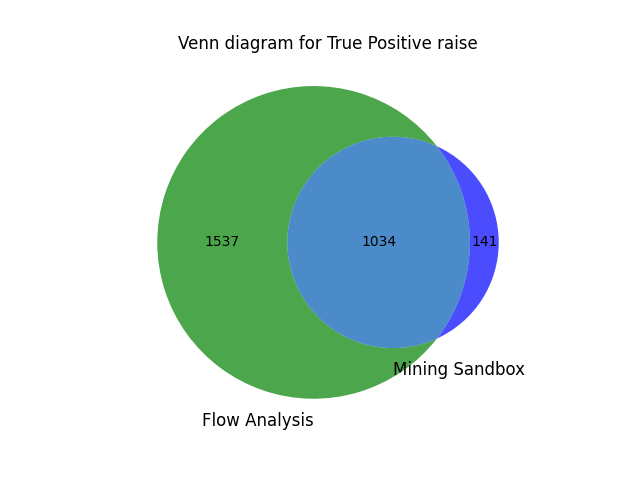
\includegraphics[width=0.5\textwidth]{image/vennTP.png} \\[\abovecaptionskip]
    \small (a) True Positive raise
  \end{tabular}

  \begin{tabular}{@{}c@{}}
    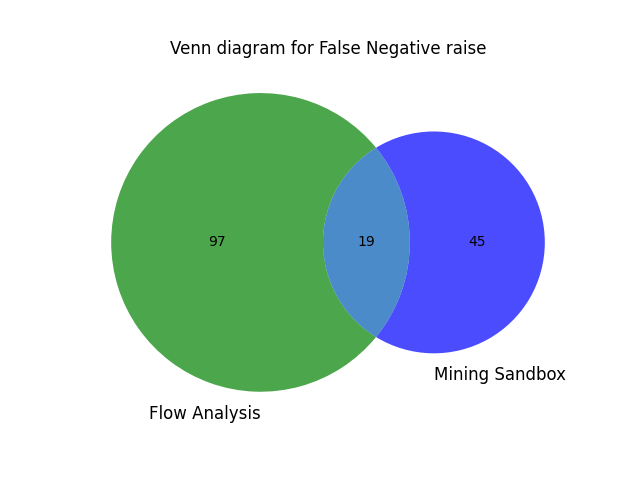
\includegraphics[width=0.5\textwidth]{image/vennFP.png} \\[\abovecaptionskip]
    \small (b) False Positive raise
  \end{tabular}
   \begin{tabular}{@{}c@{}}
    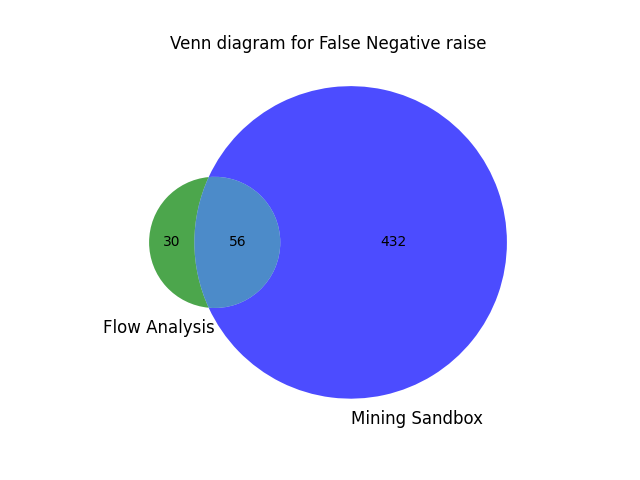
\includegraphics[width=0.5\textwidth]{image/vennFN.png} \\[\abovecaptionskip]
    \small (c) False Negative raise
  \end{tabular}

  \caption{Contribution to the final detection result}\label{fig:venn}
\end{figure}




\subsubsection{Detection Performance based on Malware Family}\label{sec:family-assessment}

In this section, we present the performance of our experiment based on malware family. Since the number of samples in each family varies, the overall detection rate is more influenced by families with larger sample sizes. However, our results become inconsistent if we use the same number of samples for each family. To resolve this issue, we present the results based on the actual number of samples from the $20$ most representative families, which account for $90.9\%$ of all malware samples tested and whose families could be labeled by \vt.

We also explored the detection rate of recent malware samples. Although their families are unknown, we demonstrated that it is possible to classify them as suspicious apps using our framework (Section~\ref{sec:unknowfamily}).


\subsubsection{Detection rate of 20 most representative malware families}\label{sec:familyDetection}


Among the $20$ most representative families, the families with the highest earnings are \gps and \dwg. Among the $69$ samples evaluated from the \dwg family, \droidxpflow flagged $66$ apps ($95.65\%$) as malicious. Despite this, the \dwg family does not have as many representative samples as the \gps family, which accounts for $46.96\%$ of all samples tested in the \fds, with $372$ samples. Of these, \droidxpflow flagged $348$ samples ($93.55$\%) as malicious. Malware belonging to the \gps family automatically connects to networks, communicates with remote servers, downloads and installs other apps or adware without the user’s knowledge\cite{DBLP:journals/jnca/WangCYYPJ19}. Due to their high network interaction, they are more easily detected by our framework, demonstrating its effectiveness in detecting samples with malicious network behaviors.

Additionally, it is worth noting that among the $20$ most representative families examined, our framework correctly identified all samples as malware in 12 families. This result demonstrates that our approach is effective for other malware families investigated as well. Table~\ref{tab:families_rate} shows the detection performance of our strategies for the $20$ most representative families. The table also classify samples from five malware categories: ad fraud, adware, spyware, trojans, and SMS malware. Most of the samples are from the adware and ad fraud categories, which aggressively display ads, generate fraudulent ad clicks, and track user behavior~\cite{DBLP:journals/spe/FallahB22}. The other categories are equally harmful and may cause financial losses through unauthorized messages (SMS malware), collect sensitive user data for malicious purposes (Spyware), or provide remote access and control over infected devices (Trojans).



\begin{table*}[h]
  \caption{Detection Rate of the $20$ most representative Families from $30\%$ tested randomly selected from \fds.}
\centering{
  \begin{tabular}{llrrr} \hline
    Category & Family & Samples & Detected  & \%  \\
    \hline

        Ad Fraud & gappusin & 372 & 348 & 93,55  \\
        ~ & dowgin & 69 & 66 & 95,65  \\
        ~ & kyvu & 4 & 4 & 100,00  \\
        Adware & revmob & 67 & 62 & 92,54  \\
        ~ & airpush & 44 & 42 & 95,45  \\
        ~ & youmi & 28 & 28 & 100,00  \\
        ~ & kuguo & 22 & 22 & 100,00  \\
        ~ & leadbolt & 15 & 15 & 100,00  \\
        ~ & adwo & 10 & 10 & 100,00  \\
        ~ & apptrack & 10 & 10 & 100,00  \\
        ~ & domob & 9 & 9 & 100,00  \\
        ~ & appsgeyser & 6 & 5 & 83,33  \\
        ~ & admogo & 6 & 5 & 83,33  \\
        ~ & pircob & 5 & 5 & 100,00  \\
        ~ & cimsci & 4 & 4 & 100,00  \\
        
        ~ & dnotua & 3 & 3 & 100,00  \\
        Spyware & igexin & 7 & 7 & 100,00  \\
        ~ & cnzz & 4 & 4 & 100,00  \\
        Trojan & torjok & 8 & 7 & 87,50  \\
        SMSmalware & smsreg & 29 & 27 & 93,10  \\

   
    \hline
  \end{tabular}
  }
  \label{tab:families_rate}
\end{table*}


\begin{finding}

Our approach proved to be efficient at malware families with high network interaction, like demonstrated at samples from \gps family, the most representative family in \fds. This demonstrates the potential of this solution in detecting samples with malicious network behaviors.

\end{finding}


\subsubsection{Detection rate of unknown malware family}\label{sec:unknowfamily}

According to \vt, among the samples from our \fds, at least two security engines identified $80$ samples as malware, but they were unable to specify their families. Since new malware emerges daily, accurately classifying recent malicious apps into their respective families is both challenging and time-consuming~\cite{DBLP:journals/compsec/WangTW21,DBLP:journals/compsec/ContiKP22}, suggesting that these are recent malware.

Although the specific families were unknown at the time of this research, our framework flagged $39$ samples ($48.75\%$) as malicious. Based on these results, we conclude that \droidxpflow can classify recent apps as malware based solely on their malicious network activity.

\begin{finding}

Even for recently malicious apps without family classification, our approach can flag them as malware based solely on their suspicious network activities.

\end{finding}







